\documentclass[conference, 12pt]{IEEEtran}
\IEEEoverridecommandlockouts
% The preceding line is only needed to identify funding in the first footnote. If that is unneeded, please comment it out.
\usepackage{cite}
\usepackage{amsmath,amssymb,amsfonts}
\usepackage{algorithmic}
\usepackage{graphicx}
\usepackage{textcomp}
\usepackage{hyperref}
\usepackage{xcolor}
\def\BibTeX{{\rm B\kern-.05em{\sc i\kern-.025em b}\kern-.08em
    T\kern-.1667em\lower.7ex\hbox{E}\kern-.125emX}}
\begin{document}

\title{Kaugummi zur Übelkeitsminderung in der Virtual Reality\\}

\author{Philipp Lauer, Denis Schlusche, Marc Zintel}

\maketitle

\begin{abstract}
Hier wird ein fantastisches Abstract stehen später
\end{abstract}

\begin{IEEEkeywords}
component, formatting, style, styling, insert
\end{IEEEkeywords}

\section{Einleitung}
Viele Menschen, die schon einmal in die Virtual Reality eingetaucht sind, empfinden ein Gefühl der Benommenheit und Übelkeit. Diese Übelkeit wird auch Motion Sickness oder Virtual Reality Krankheit genannt. Ein Ansatz, diese Motion Sickness zu umgehen, ist es Ablenkung zu schaffen. Eine solche Ablenkung wird im Folgenden durch das Kauen eines Kaugummis umgesetzt. Hierdurch soll der Kiefer in Bewegung gehalten und eine angenehme Ablenkung durch den Geschmack erzeugt werden. Es werden 20 Probanden in A/B-Tests gefordert, in einer Virtual Realtiy-Anwendung sechs Minuten zu verbringen und dabei stets neue Dinge zu suchen. Die Anwendung ist ein Nachbau der US-Amerikanischen Großstadt San Francisco, weshalb es sinnvoll ist, markante Bauwerke als Ziel der Suche auzuwählen. 

\section{Versuch}
\subsection{Idee}
Die grundsätzliche Idee hinter dem Versuch lautet: Durch das Kauen von Kaugummi wird Menschen in der Virtual Reality weniger schlecht.
Diese Idee basiert darauf, dass durch das Kauen eine stetige Bewegung des Kiefers und Kopfes ausgelöst wird, welche das Gehirn zu einem gewissen Maß ablenkt. Dadurch soll das Auftreten von Motion Sickness verringert beziehungsweise gemildert werden. 
\\
\\
Statistisch formulieren wir das so:

Die beiden Stichproben haben unterschiedliche Erwartungswerte in den Beurteilungen. Die Mittelwerte der beiden Stichproben sind verschieden, der aus der Ohne-Kaugummi-Gruppe ist kleiner als der aus der Mit-Kaugummi-Gruppe. Neben den beiden Stichproben mit Fragen und Antworten auf einer Likert-Skala gibt es einen weiteren Datensatz mit Meta-Angaben zu den Probanden. Dabei ist die Nummerierung der Probanden in allen drei Dateien gleich.

Die Stichprobe Mit- und Ohne-Kaugummi sind verbundene Stichproben.

\subsection{Versuchsaufbau}
Es werden 20 Probanden in einem A/B-Test in einer Virtual Reality-Anwendung zwei Versuchsdurchläufe absolvieren. Dabei werden die Probanden von eins bis zwanzig durchnummeriert. Die Hälfte der Probanden mit ungeraden Nummern startet mit Kaugummi, die mit geraden ohne. Der zweite Durchlauf ist jeweils entgegengesetzt. Ein Versuchsdurchlauf dauert sechs Minuten. Nach jedem Durchlauf werden die Probanden gebeten, einen vorgefertigten MSAQ-Fragebogen auszufüllen. Dieser soll die Gefühle der Probanden widerspiegeln und zeigen, in welchem Versuchsdurchlauf eine angenehmere Durchführung der Aufgaben möglich war. Zur Durchführung wird die HTC-Vive Pro, inklusive zweier Controller verwendet. Die Anwendung ist ein Nachbau von San Francisco, in dem sich der Proband frei bewegen kann. Darin sollen markante Punkte gefunden werden, darunter die Golden Gate Bridge, ein Fußballstadion, sowie ein Baseballstadion. Im Anschluss an diese vorhandenen Orte bekamen die Probanden die Aufgabe, einen etwa hausgroßen, grünen Godzilla zu suchen, der beim Start des Programmes an der Golden Gate Bridge losging. Diese Aufgabe sollte auch nach Vollendung der gefundenen Bauwerke den Probanden zum Suchen und zur Bewegung animieren. Während der Versuchsdurchläufe wird jeweils die Zeit in Bewegung und die Standzeit aufgezeichnet, sodass auch diese Variable erfasst werden kann. Außerdem wird der Proband vor dem Versuch nach seiner bisherigen Erfahrung mit Virtual Realtiy Anwendungen gefragt, sodass sichergestellt werden kann, dass erfahrene Nutzer gegebenenfalls ermittelt werden können, falls dies die Statistik verfälscht. 
\\
\begin{figure}
	\centering
	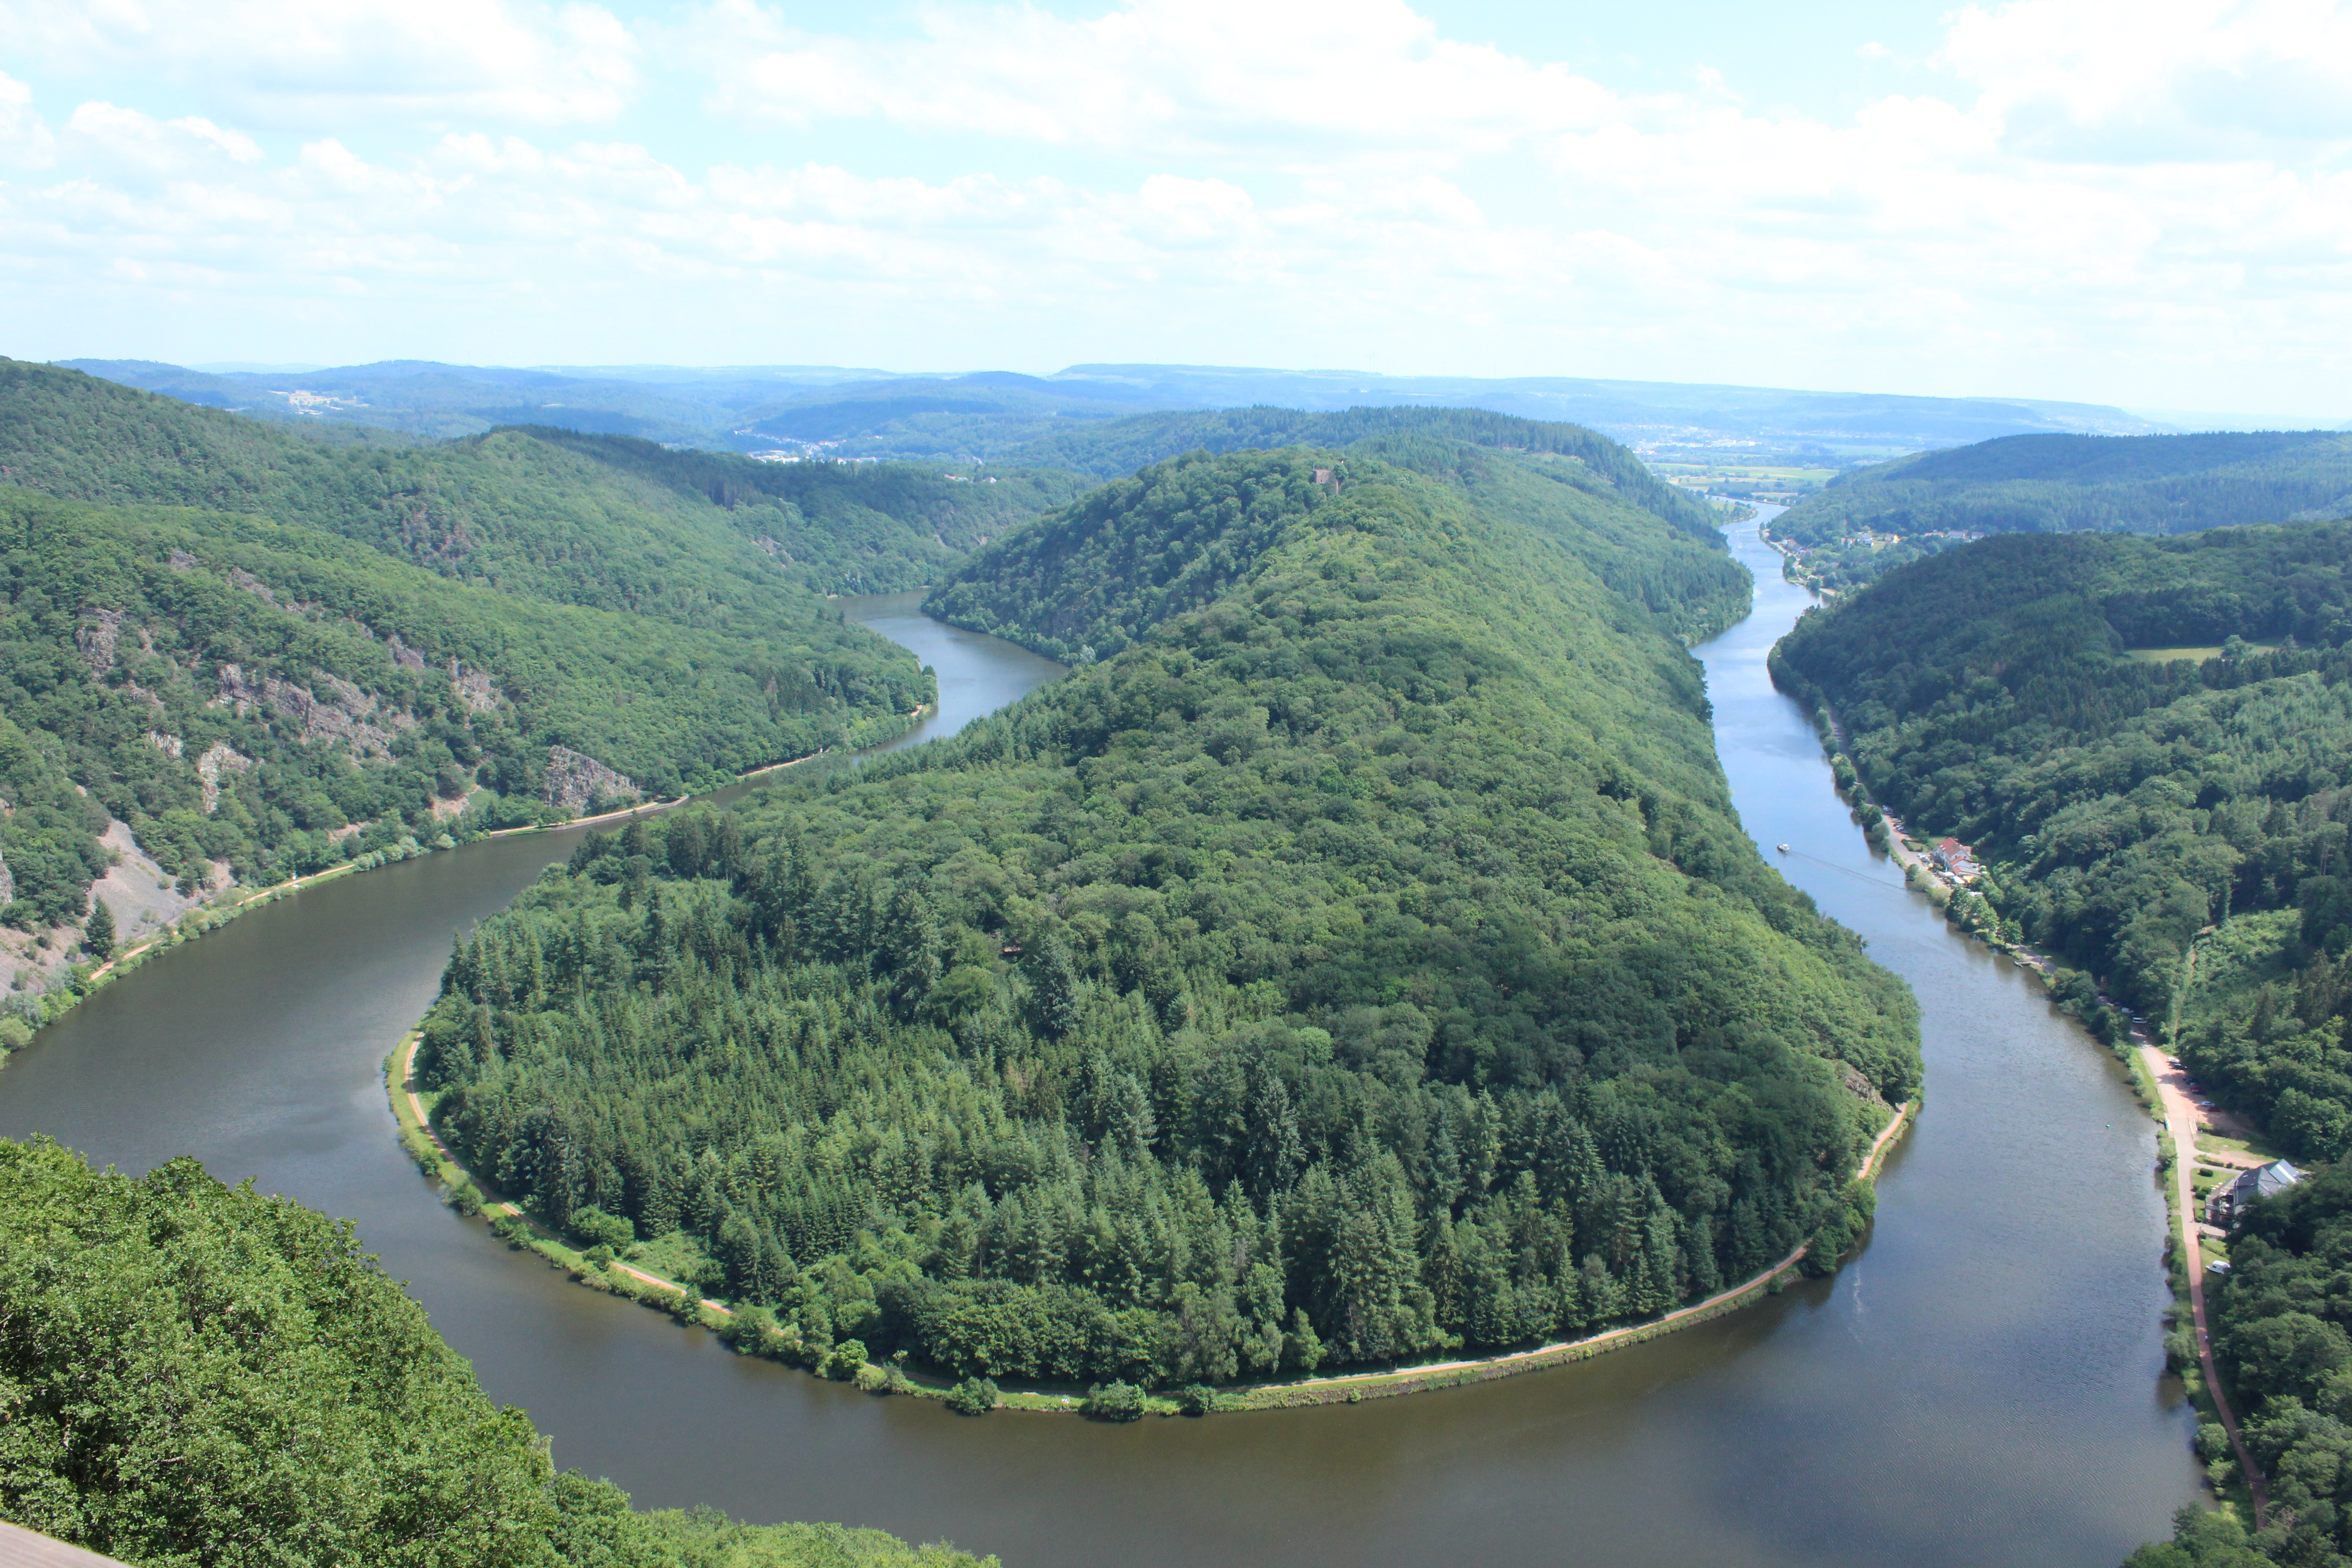
\includegraphics[width=0.5\textwidth]{sanfrancisco.jpg}
	\caption{Screenshot aus der Anwendung}
	\label{img:screenshot}
\end{figure}



\section{Auswertung der Daten}




\begin{figure}
	\centering
	\includegraphics[width=0.5\textwidth]{Mittelwert3-17.png}
	\caption{Mittelwerte der Fragen FB3-FB17}
	\label{img:mittelwerte}
\end{figure}



\section{Ergebnis}



\section{Fazit}



\begin{thebibliography}{00}
\bibitem{b1} M. Brill: YouTube Playlist Datenanalyse, unter: {\url{https://www.youtube.com/watch?v=efP9IYVKqA0&list=PL-8_avPKkCnreV8olzMEQxwSrzagoVpmb}}
\bibitem{b2} L. Fahrmeir, R. Künster, I. Pigeot, G. Tutz: Statistik - Der Weg zur Datenanalyse, Springer, 2007.
\bibitem{b3} Wickham, Grolemund: R for Data Science, O'Reilly, 2017.
\bibitem{b4} Kabacoff: R in Action, Manning, 2015.
\bibitem{b5} Wickham: Advanced R, CRC Press, 2014.
\end{thebibliography}
\end{document}
